
% This LaTeX was auto-generated from MATLAB code.
% To make changes, update the MATLAB code and republish this document.

\documentclass{article}
\usepackage{graphicx}
\usepackage{color}

\sloppy
\definecolor{lightgray}{gray}{0.5}
\setlength{\parindent}{0pt}

\begin{document}

    
    \begin{verbatim}
R = 1000;
L = 0.2;
C = 0.05;

G = tf([R],[R*C*L, R^2+C, R])
G = 30*G;
step(G);

ylabel('Output Voltage [V]')
title('Step Response of Q7.19')
\end{verbatim}

        \color{lightgray} \begin{verbatim}
G =
 
           1000
  ----------------------
  10 s^2 + 1e06 s + 1000
 
Continuous-time transfer function.

\end{verbatim} \color{black}
    
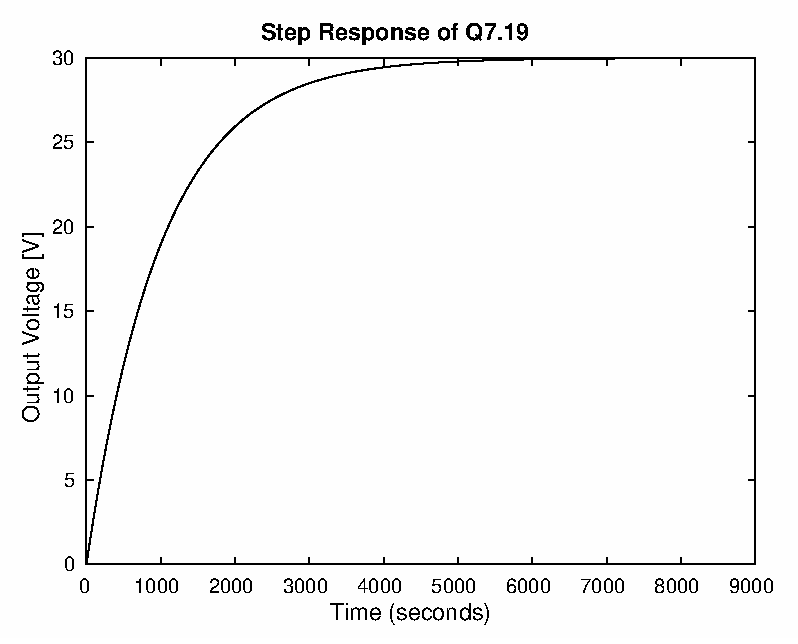
\includegraphics [width=4in]{Q7_19_01.eps}



\end{document}
    
